\documentclass[12pt]{article}

\usepackage[utf8]{inputenc}
\usepackage{latexsym,amsfonts,amssymb,amsthm,amsmath, graphicx, float, hyperref, caption, breakurl, url}

\setlength{\parindent}{0in}
\setlength{\oddsidemargin}{0in}
\setlength{\textwidth}{6.5in}
\setlength{\textheight}{8.8in}
\setlength{\topmargin}{-0.5in}
\setlength{\headheight}{18pt}


\title{Assignment 1 — Applied Algorithms, T. II/2024–25}
\author{Austin Jetrin Maddison 6481268}

\begin{document}
	% \small
	
	\maketitle
	
	\vspace{0.5in}
	
	\subsection*{Problem 1. Las Vegas and Monte Carlo}
	
	
	a.i) We want to show the probablity of running time of Monte Carlo is atleast the worst running time which is $4f(n)$. We can use markov inqualities to bound it..
	\\

	\begin{align*}
		\textbf{P}(X \le \lambda ) & \le \frac{ E [ X ] }{ \lambda }\\
	\end{align*}

	\begin{align*}
		\textbf{P}(T(n) \le 4f(n) ) & \le \frac{f(n)}{4f(n)}\\
								    & \le \frac{1}{4}		
	\end{align*}
	
	a.ii) The worse-case running time happens at most 1/4 which produces incorrect answers. We can get the complement of the last answer...    

	\begin{align*}
		1 - \textbf{P}(T(n) \le 4f(n) ) &  \le 1 - \frac{1}{4} = \frac{3}{4}
	\end{align*}
	
	b.i) The LV algorithm running time is described as the follwing. Each iteration requires running A to produce an answer then run C to check the answer. So the running time for each trial is...
	
	\begin{align*}
		\text{1 iteration running time of LV} = f(n) + g(n)
	\end{align*}

	So the question is what is the expected iterations needed to run LV to get a correct answer. If p is the probablity of success then the expected $1/p$.

	\begin{align*}
		\text{Running time of LV} = \frac{1}{p}(f(n) + g(n))
	\end{align*}

	\vspace{2in} %Leave space for comments!
	
	
	\subsection*{Problem 2. Chernoff-Hoeffding With Bounds}
	2.1)
	\begin{align*}
		\mathrm{Pr}[X &> (1+\beta)\mu]\leq\exp\left(-\frac{\beta^{2}}{2+\beta}\mu H\right) \\
		\mathrm{Pr}[X &> (1+\varepsilon)\mu H]\leq\exp\left(-\frac{\varepsilon^{2}}{2+\varepsilon}\mu H\right)
	\end{align*}

	\begin{align*}
		(1 + \epsilon) \mu_{H} &= (1 + \beta) \mu \\
		\frac{\mu_{H}}{\mu} &= \frac{1 + \epsilon}{1 + \beta}\\
		% \beta $= \frac{\mu_{H}(1 + \epsilon)}{\mu}\\
	\end{align*}


	2.2)
	\begin{align*}
		\mathrm{Pr}[X &> (1+\beta)\mu]\leq\exp\left(-\frac{\beta^{2}}{2+\beta}\mu H\right) \\
		\mathrm{Pr}[X &> (1+\varepsilon)\mu H]\leq\exp\left(-\frac{\varepsilon^{2}}{2+\varepsilon}\mu H\right)
	\end{align*}

	\begin{align*}
		(1 + \epsilon) \mu_{H} &= (1 + \beta) \mu \\
		\frac{\mu_{H}}{\mu} &= \frac{1 + \epsilon}{1 + \beta}\\
		% \beta $= \frac{\mu_{H}(1 + \epsilon)}{\mu}\\
	\end{align*}

	2.3)
	\begin{align*}
		\mathrm{Pr}[X &> (1+\beta)\mu]\leq\exp\left(-\frac{\beta^{2}}{2+\beta}\mu H\right) \\
		\mathrm{Pr}[X &> (1+\varepsilon)\mu H]\leq\exp\left(-\frac{\varepsilon^{2}}{2+\varepsilon}\mu H\right)
	\end{align*}

	\begin{align*}
		(1 + \epsilon) \mu_{H} &= (1 + \beta) \mu \\
		\frac{\mu_{H}}{\mu} &= \frac{1 + \epsilon}{1 + \beta}\\
		% \beta $= \frac{\mu_{H}(1 + \epsilon)}{\mu}\\
	\end{align*}
	
	2.4)
	\begin{align*}
		\mathrm{Pr}[X &> (1+\beta)\mu]\leq\exp\left(-\frac{\beta^{2}}{2+\beta}\mu H\right) \\
		\mathrm{Pr}[X &> (1+\varepsilon)\mu H]\leq\exp\left(-\frac{\varepsilon^{2}}{2+\varepsilon}\mu H\right)
	\end{align*}

	\begin{align*}
		(1 + \epsilon) \mu_{H} &= (1 + \beta) \mu \\
		\frac{\mu_{H}}{\mu} &= \frac{1 + \epsilon}{1 + \beta}\\
		% \beta $= \frac{\mu_{H}(1 + \epsilon)}{\mu}\\
	\end{align*}
	\vspace{2in} %Leave space for comments!
	
	
	\subsection*{Problem 3. Rescaling Trick}
	(Statement of problem goes here.)\\
	
	\begin{proof}
		(Type your proof here.)
	\end{proof}
	
	\vspace{2in} %Leave space for comments!
	
	
	
	\subsection*{Problem 4. $x^2$ With $\pi$ Degrees of Freedom}
	(Statement of problem goes here.)\\
	
	\begin{proof}
		(Type your proof here.)
	\end{proof}
	
	\vspace{2in} %Leave space for comments!
	
	
	\subsection*{Problem 5. Simple Samplers.}
	(Statement of problem goes here.)\\
	
	\begin{proof}
		(Type your proof here.)
	\end{proof}
	
	\vspace{2in} %Leave space for comments!
	
	
	\subsection*{Problem 6. Median of Means}
	(Statement of problem goes here.)\\
	
	\begin{proof}
		(Type your proof here.)
	\end{proof}
	
	\vspace{2in} %Leave space for comments!
	
	
	\subsection*{Problem 7. Skip List}
	\vspace{20pt}
	\subsubsection*{Experimental Setup}
	Conducted our benchmarks using Google Benchmark~\cite{google-bench} on a system with the following hardware specifications:

\begin{itemize}
	\small
    \item \textbf{Processor}: 11th Gen Intel(R) Core(TM) i7-11370H 4C/8T CPU @ 3.3 GHz
    \item \textbf{Cache Hierarchy}:
    \begin{itemize}
        \item L1 Data: 48 KiB per core (\(\times 4\))
        \item L1 Instruction: 32 KiB per core (\(\times 4\))
        \item L2 Unified: 1280 KiB per core (\(\times 4\))
        \item L3 Unified: 12,288 KiB (shared)
    \end{itemize}
\end{itemize}

All benchmarks were compiled using \texttt{-Ox} optimization level with \texttt{MSVC} (version 19.42.34436) and executed in a single-threaded environment to minimize external interference. Memory usage was measured using the Windows API \texttt{GetProcessMemory()}~\cite{getprocessmemoryinfo}.\\

\subsubsection*{Questions And Experiments}
	
a.1) Can we perform count coin tosses differently and is the alternative better?

\begin{figure}[H]
	\centering
	\begin{minipage}{0.32\textwidth}
		\centering
		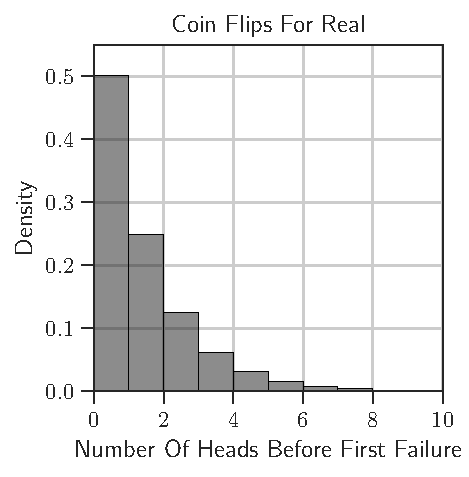
\includegraphics[width=\linewidth]{../notebook/plot/coin_flips_for_real.pdf}
		\label{fig:coin_flips_for_real}
	\end{minipage}\hfill
	\begin{minipage}{0.32\textwidth}
		\centering
		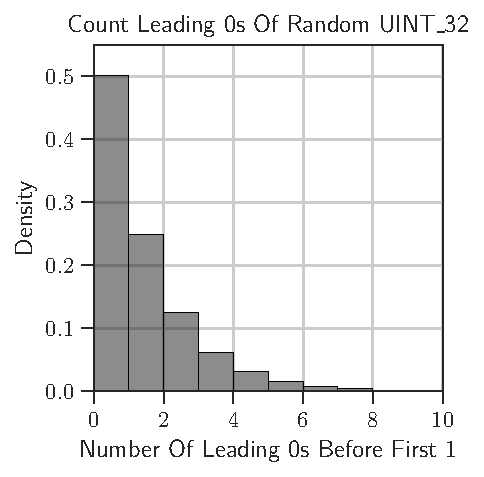
\includegraphics[width=\linewidth]{../notebook/plot/count_leading_0s_of_random_uint_32.pdf}
		\label{fig:coin_flips_count_leading}
	\end{minipage}\hfill
	\begin{minipage}{0.32\textwidth}
		\centering
		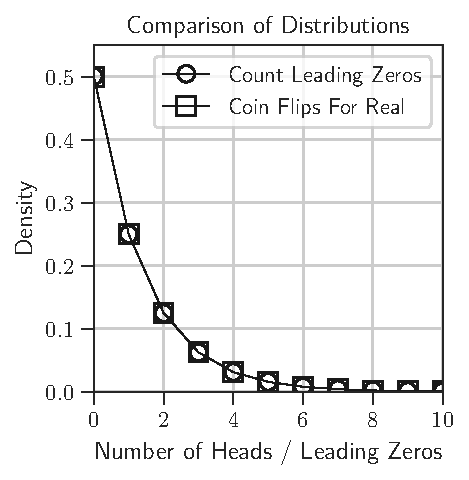
\includegraphics[width=\linewidth]{../notebook/plot/comparison_of_distributions.pdf}
		\label{fig:coin_flips_comparison}
	\end{minipage}
\end{figure}


\begin{table}[h]
	\centering
	\small
	\begin{tabular}{lrrr}
		\hline
		\textbf{Benchmark} & \textbf{Time (ns)} & \textbf{CPU (ns)} & \textbf{Iterations} \\
		\hline
		Coin Flip For Real & 29.8 & 29.3 & 22,400,000 \\
		\hline
		Coin Flip Count Leading 0s & 5.11 & 4.87 & 144,516,129 \\
	\end{tabular}
	\caption{Benchmark results comparing different coin flip implementations.}
	\label{tab:benchmark_results}
\end{table}


a.2) How to define vertical nodes withoud the downsides of introducing linked-list like overhead? \\

This is an awfully convenient question, because it is, I chose the question as an outlet to describe how I got to my current implementation of skip list. My first implementation of skip list was almost 2 weeks ago was horrendously slow. It took seconds to insert 1 million keys, never mind trying to insert 10s of millions of keys. It was so frustrating, I couldn't pinpoint exactly what was causing the bottleneck. The code was text-book, simple node struct, search for the insertion point, and stitch the new node/nodes into place.
\\\\
After dilly dallying with debuggers and profilers, I thought that traversal was what was slowing everything down. Instead of using a linked-list to extend higher keys I thought of using an array instead as it is more cache friendly and might help solve the problem. I didn't have to store keys at every-level and vertical references. Since the data is more 'packed' I thought maybe it would solve the long traversal times.
\\\\
At last I felt that inserting keys were faster however it still took almost a second to insert a million keys. After sulking in the group chat, Jorn asks whether I got my implementation ideas from a particular stack-overflow thread \cite{stack-overflow} as I had that vertical array going on. I sure didn't but I was surprised to see in many ways the shape of their function was kinda the same. We came to similar conclusions on implementation. However one thing that stood out in this implementation the author took special care in allocating nodes. They used a custom allocator, and allocated arrays manually. Their results were blazingly fast!
\\\\
For my array data-structure I used \texttt{std::vector}, it was a big mistake, vectors have all kinds of fancy stuff to make them safe and easy to use. All the added indirection vector brought killed the performance of my skip-list. After swapping out std::vector to directly allocating the memory  like the author in that stack-overflow thread, the speed was finally bearable to insert $2^{22}$ keys.
\\\\

\pagebreak

a.3) How does it perform against a reputable ordered map?\\


\noindent
\begin{minipage}{0.45\textwidth}
    \centering
	\resizebox{1\textwidth}{!}{%
		\begin{tabular}{rrr}
		\hline
		\multicolumn{3}{c}{\textbf{Skip List Insertion}} \\ \hline
		n             & CPU Time (ms)      & Memory Usage (KB)      \\ \hline
		8       & 1.14E-04 & 0      \\
		16      & 1.76E-04 & 0      \\
		32      & 5.78E-04 & 0      \\
		64      & 1.20E-03 & 0      \\
		128     & 3.25E-03 & 0      \\
		256     & 6.63E-03 & 0      \\
		512     & 1.60E-02 & 0      \\
		1024    & 6.98E-02 & 32     \\
		2048    & 2.00E-01 & 72     \\
		4096    & 4.39E-01 & 208    \\
		8192    & 1.20E+00 & 444    \\
		16384   & 2.54E+00 & 884    \\
		32768   & 6.56E+00 & 1724   \\
		65536   & 1.75E+01 & 3436   \\
		131072  & 4.97E+01 & 6988   \\
		262144  & 1.88E+02 & 15048  \\
		524288  & 6.72E+02 & 30228  \\
		524288  & 6.88E+02 & 30172  \\
		1048576 & 1.69E+03 & 60384  \\
		2097152 & 4.42E+03 & 120756 \\
		4194304 & 1.14E+04 & 241416 \\
		8388608 & 2.81E+04 & 483244  \\ \hline
		\end{tabular}
	}
    % \captionof{table}{First Table}
\end{minipage}%
\hfill
\begin{minipage}{0.45\textwidth}
    \centering
	\resizebox{1.0\textwidth}{!}{%
		\begin{tabular}{rrr}
		\hline
		\multicolumn{3}{c}{\textbf{Ordered Map Insertion}} \\ \hline
		n             & CPU Time (ms)      & Memory Usage (KB)      \\ \hline
		8       & 0.00E+00 & 0      \\
		16      & 0.00E+00 & 0      \\
		32      & 0.00E+00 & 0      \\
		64      & 1.32E+01 & 0      \\
		128     & 4.73E+00 & 0      \\
		256     & 1.25E+01 & 0      \\
		512     & 0.00E+00 & 0      \\
		1024    & 5.78E+00 & 0      \\
		2048    & 8.72E+00 & 0      \\
		4096    & 1.45E+01 & 0      \\
		8192    & 2.78E+01 & 0      \\
		16384   & 4.94E+01 & 0      \\
		32768   & 4.88E+01 & 0      \\
		65536   & 5.31E+01 & 68     \\
		131072  & 1.20E+02 & 136    \\
		262144  & 3.33E+02 & 11864  \\
		524288  & 5.26E+02 & 204    \\
		524288  & 5.23E+02 & 336    \\
		1048576 & 8.28E+02 & 24396  \\
		2097152 & 2.08E+03 & 98332  \\
		4194304 & 5.08E+03 & 197080 \\
		8388608 & 1.25E+04 & 394916 \\ \hline
		\end{tabular}
		}
\end{minipage}%
\vspace{14pt}
\begin{minipage}{0.45\textwidth}
    \centering
	\resizebox{1\textwidth}{!}{%
		\begin{tabular}{rrr}
		\hline
		\multicolumn{3}{c}{\textbf{Skip List Search}} \\ \hline
		n             & CPU Time (ms)      & Memory Usage (KB)      \\ \hline
		8       & 2.90E-05 & 0      \\
		16      & 8.50E-05 & 0      \\
		32      & 3.49E-04 & 0      \\
		64      & 6.10E-04 & 0      \\
		128     & 1.22E-03 & 0      \\
		256     & 2.70E-03 & 0      \\
		512     & 7.12E-03 & 0      \\
		1024    & 6.00E-02 & 0      \\
		2048    & 1.57E-01 & 32     \\
		4096    & 3.99E-01 & 28     \\
		8192    & 9.83E-01 & 156    \\
		16384   & 2.68E+00 & 520    \\
		32768   & 6.28E+00 & 1476   \\
		65536   & 1.67E+01 & 3320   \\
		131072  & 4.69E+01 & 6972   \\
		262144  & 2.15E+02 & 14604  \\
		524288  & 5.31E+02 & 29776  \\
		524288  & 5.63E+02 & 29708  \\
		1048576 & 1.66E+03 & 60032  \\
		2097152 & 3.95E+03 & 120340 \\
		4194304 & 9.83E+03 & 241212 \\
		8388608 & 2.36E+04 & 482876  \\ \hline
		\end{tabular}
	}
    % \captionof{table}{First Table}
\end{minipage}%
\hfill
\begin{minipage}{0.45\textwidth}
    \centering
	\resizebox{1.0\textwidth}{!}{%
		\begin{tabular}{rrr}
		\hline
		\multicolumn{3}{c}{\textbf{Ordered Map Search}} \\ \hline
		n             & CPU Time (ms)      & Memory Usage (KB)      \\ \hline
		8       & 3.20E-05 & 0      \\
		16      & 9.40E-05 & 0      \\
		32      & 2.00E-04 & 0      \\
		64      & 4.30E-04 & 0      \\
		128     & 9.84E-04 & 0      \\
		256     & 2.25E-03 & 0      \\
		512     & 6.70E-03 & 0      \\
		1024    & 3.84E-02 & 0      \\
		2048    & 1.09E-01 & 0      \\
		4096    & 2.51E-01 & 0      \\
		8192    & 6.14E-01 & 0      \\
		16384   & 1.38E+00 & 64     \\
		32768   & 4.62E+00 & 0      \\
		65536   & 1.00E+01 & 32     \\
		131072  & 2.40E+01 & 0      \\
		262144  & 8.48E+01 & 204    \\
		524288  & 2.73E+02 & 204    \\
		524288  & 2.73E+02 & 68     \\
		1048576 & 8.91E+02 & 23996  \\
		2097152 & 2.19E+03 & 49152  \\
		4194304 & 5.45E+03 & 98832  \\
		8388608 & 1.31E+04 & 290012 \\ \hline
		\end{tabular}
		}
\end{minipage}%


\begin{figure}[H]
	\centering

	\begin{minipage}{0.32\textwidth}
		\centering
		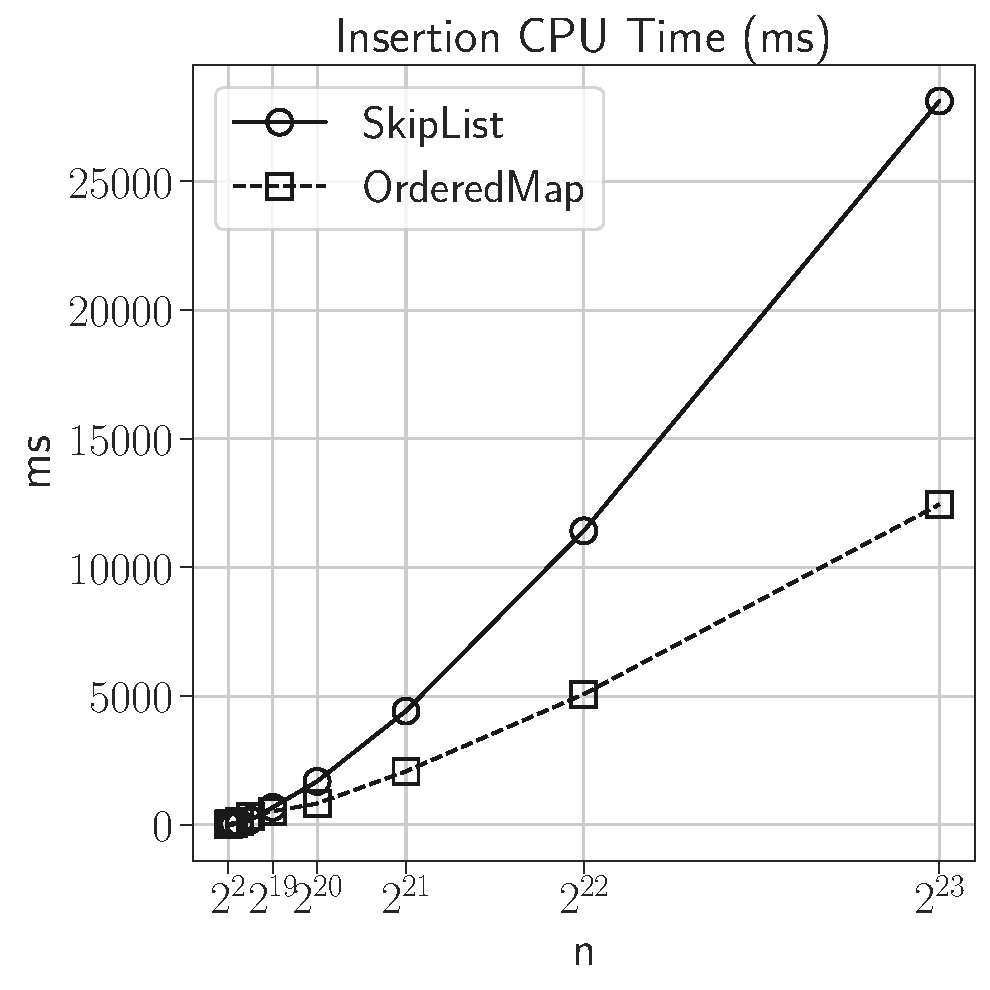
\includegraphics[width=\linewidth]{../notebook/plot/sl_insertion_cpu_time_(ms).pdf}
		\label{fig:cpu_time}
	\end{minipage}\hfill
	\begin{minipage}{0.32\textwidth}
		\centering
		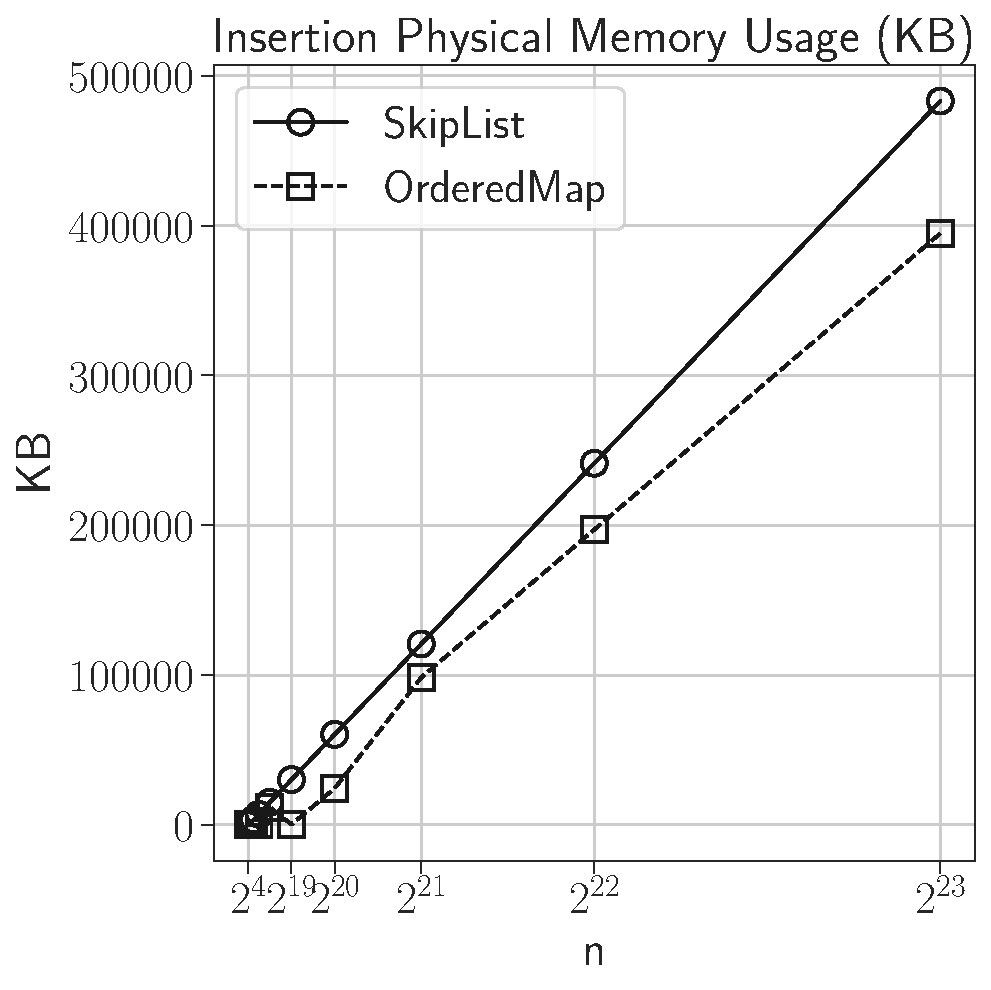
\includegraphics[width=\linewidth]{../notebook/plot/sl_insertion_physical_memory_usage_(kb).pdf}
		\label{fig:physical_memory}
	\end{minipage}\hfill\
	\begin{minipage}{0.32\textwidth}
		\centering
		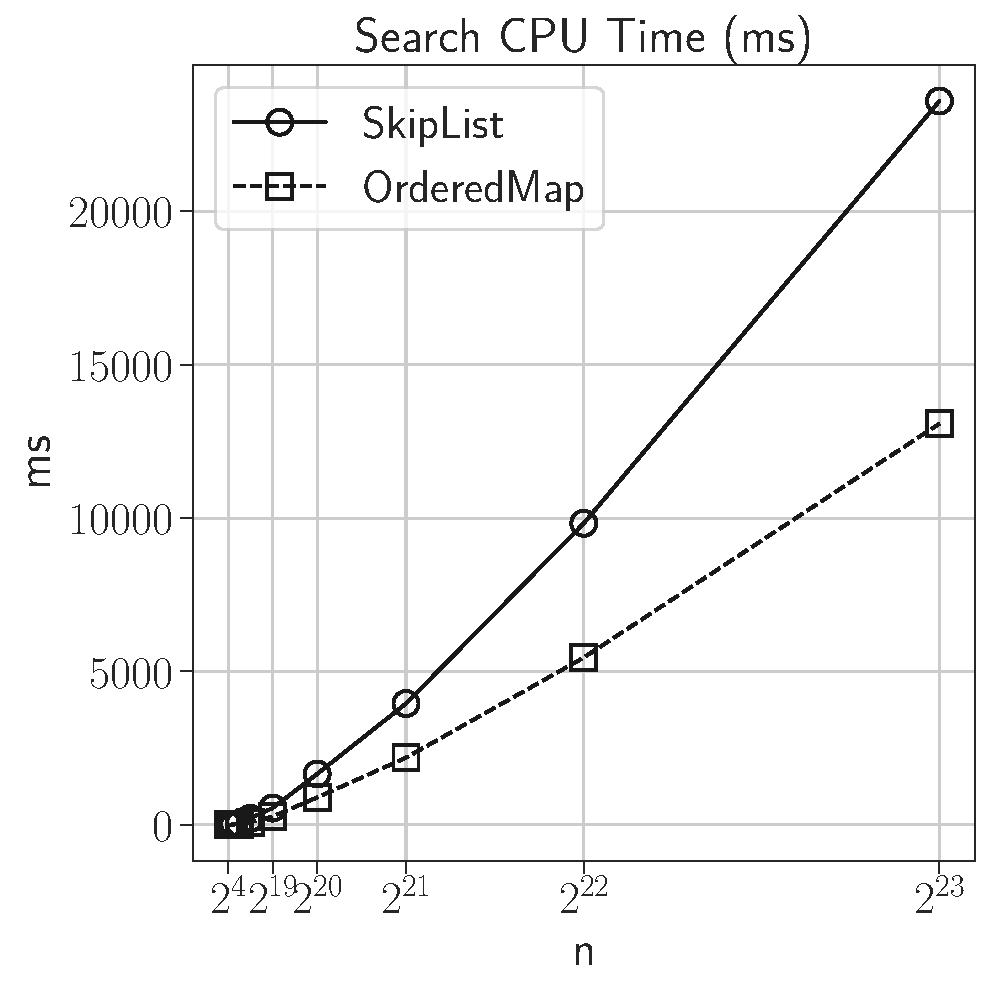
\includegraphics[width=\linewidth]{../notebook/plot/sl_search_cpu_time_(ms).pdf}
		\label{fig:physical_memory}
	\end{minipage}\hfill
	\caption{CPU Time and Memory Usage of Skip List and Ordered Map.}
\end{figure}

\begin{figure}[H]
	\centering

	\begin{minipage}{0.32\textwidth}
		\centering
		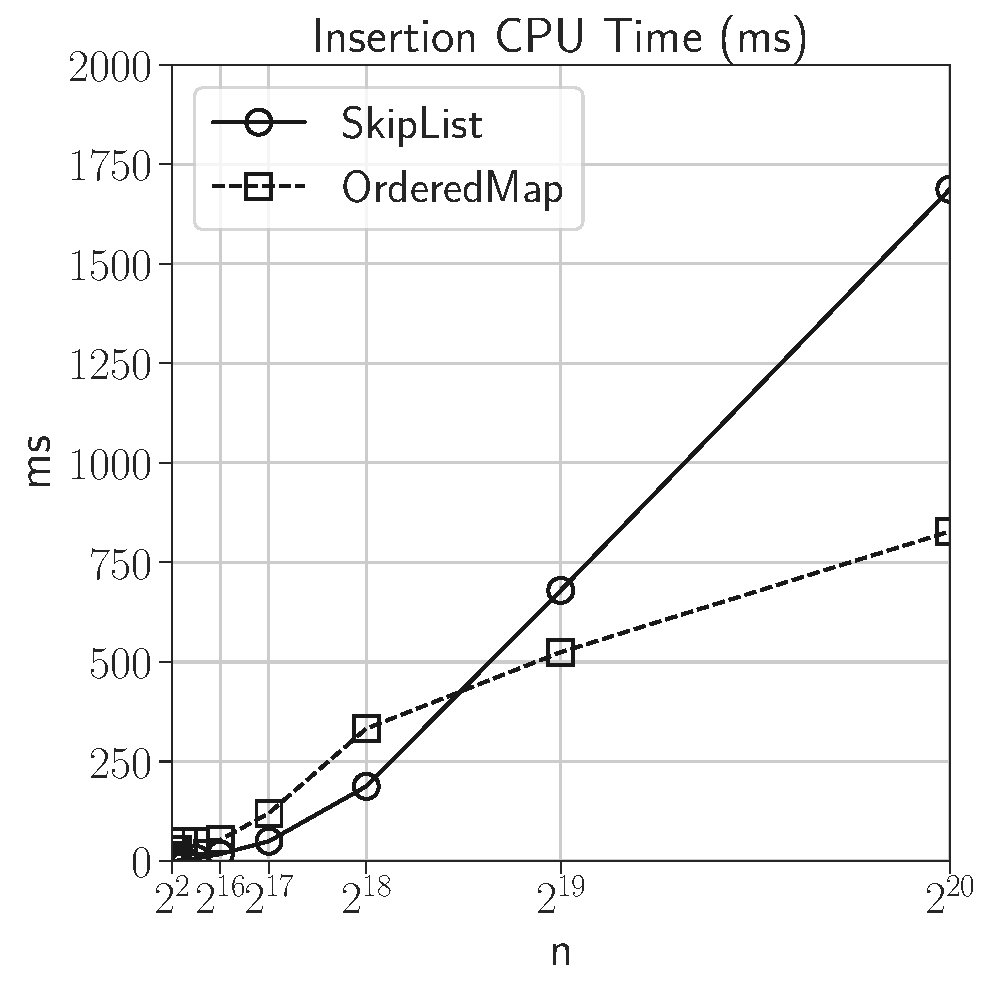
\includegraphics[width=\linewidth]{../notebook/plot/sl_liminsertion_cpu_time_(ms).pdf}
		\label{fig:cpu_time}
	\end{minipage}\hfill
	\begin{minipage}{0.32\textwidth}
		\centering
		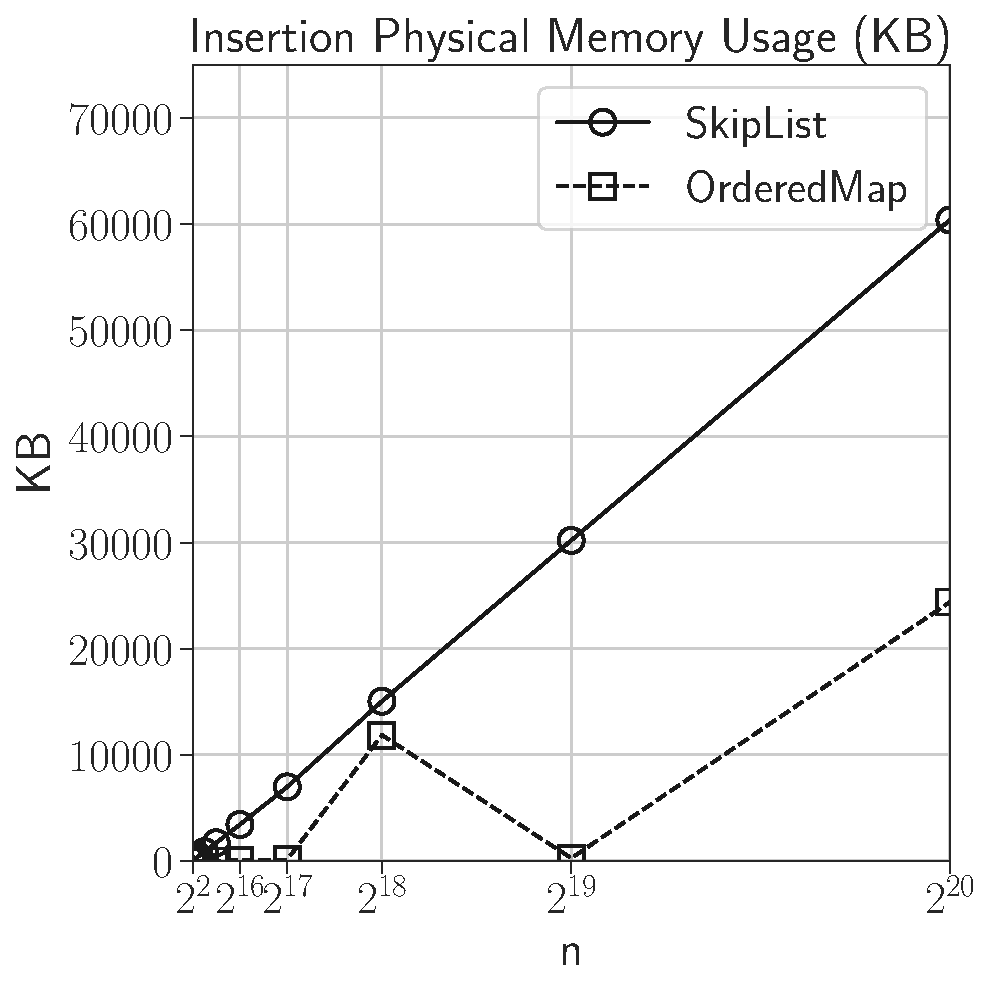
\includegraphics[width=\linewidth]{../notebook/plot/sl_liminsertion_physical_memory_usage_(kb).pdf}
		\label{fig:physical_memory}
	\end{minipage}\hfill\
	\begin{minipage}{0.32\textwidth}
		\centering
		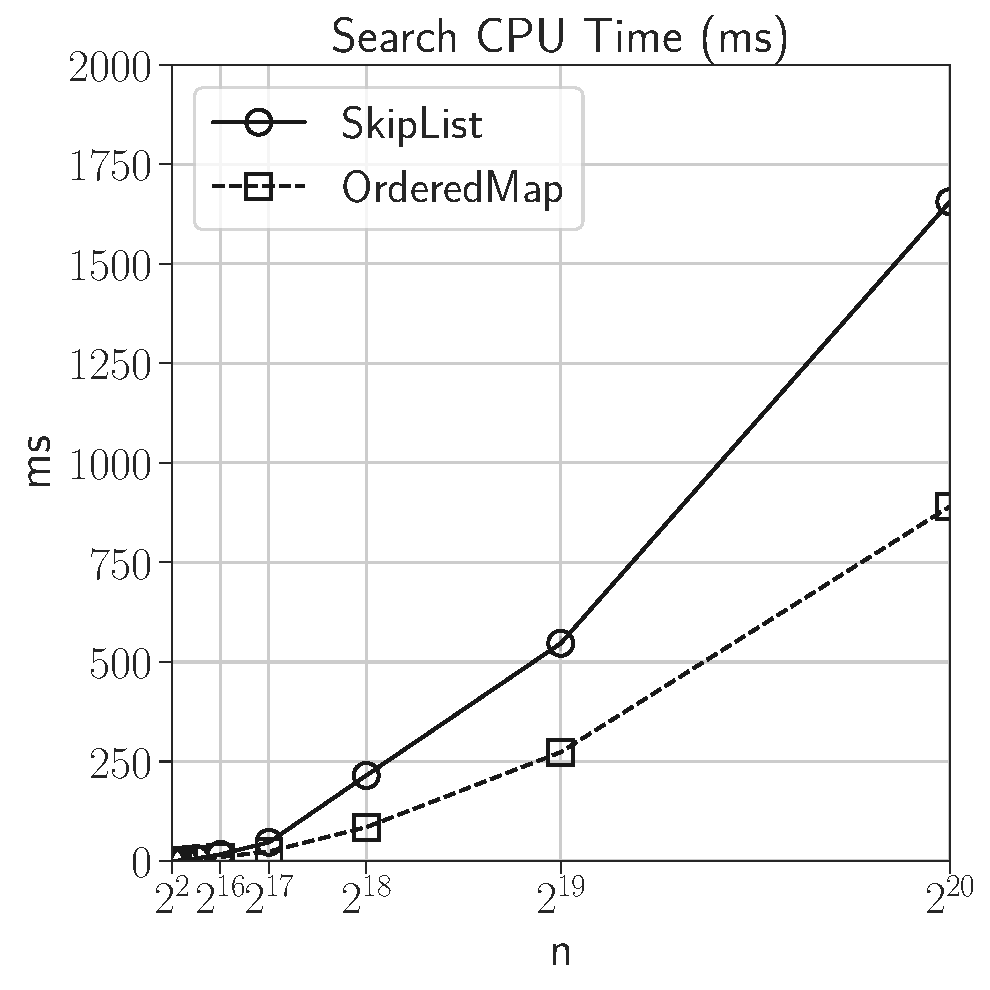
\includegraphics[width=\linewidth]{../notebook/plot/sl_limsearch_cpu_time_(ms).pdf}
		\label{fig:physical_memory}
	\end{minipage}\hfill
	\caption{Crop of Figure 1.}
\end{figure}


\pagebreak
Q4.) How might varying max height change performance of Skip List?\\

\noindent
\begin{minipage}{0.5\textwidth}
    \centering
	\resizebox{1\textwidth}{!}{%
		\begin{tabular}{rrr}
		\hline
		\multicolumn{3}{c}{\textbf{Skip List Insertion}} \\ \hline
		Max Level             & CPU Time (ms)      & Memory Usage (KB)      \\ \hline
		2  & 3.03E+04 & 6888 \\
		4  & 2.91E+03 & 7232 \\
		6  & 7.66E+02 & 7424 \\
		8  & 2.97E+02 & 7480 \\
		10 & 1.32E+02 & 7456 \\
		12 & 5.86E+01 & 7424 \\
		14 & 4.69E+01 & 7416 \\
		16 & 6.53E+01 & 7404 \\
		18 & 5.40E+01 & 7440 \\
		20 & 5.00E+01 & 7484 \\
		22 & 4.69E+01 & 7520 \\
		24 & 5.16E+01 & 7420 \\
		26 & 4.98E+01 & 7404 \\
		28 & 5.16E+01 & 7388 \\
		30 & 4.55E+01 & 7420 \\
		32 & 4.83E+01 & 7500  \\ \hline
		\end{tabular}
	}
    % \captionof{table}{First Table}
\end{minipage}%
\hfill
\begin{minipage}{0.5\textwidth}
    \centering
	\resizebox{1.0\textwidth}{!}{%
		\begin{tabular}{rrr}
		\hline
		\multicolumn{3}{c}{\textbf{Skip List Map Search}} \\ \hline
		Max Level   & CPU Time (ms)      & Memory Usage (KB)      \\ \hline
		2  & 3.03E+04 & 6888 \\
		4  & 2.91E+03 & 7232 \\
		6  & 7.66E+02 & 7424 \\
		8  & 2.97E+02 & 7480 \\
		10 & 1.32E+02 & 7456 \\
		12 & 5.86E+01 & 7424 \\
		14 & 4.69E+01 & 7416 \\
		16 & 6.53E+01 & 7404 \\
		18 & 5.40E+01 & 7440 \\
		20 & 5.00E+01 & 7484 \\
		22 & 4.69E+01 & 7520 \\
		24 & 5.16E+01 & 7420 \\
		26 & 4.98E+01 & 7404 \\
		28 & 5.16E+01 & 7388 \\
		30 & 4.55E+01 & 7420 \\
		32 & 4.83E+01 & 7500 \\ \hline
		\end{tabular}
		}
\end{minipage}%

\begin{figure}[H]
	\centering
	\begin{minipage}{0.32\textwidth}
		\centering
		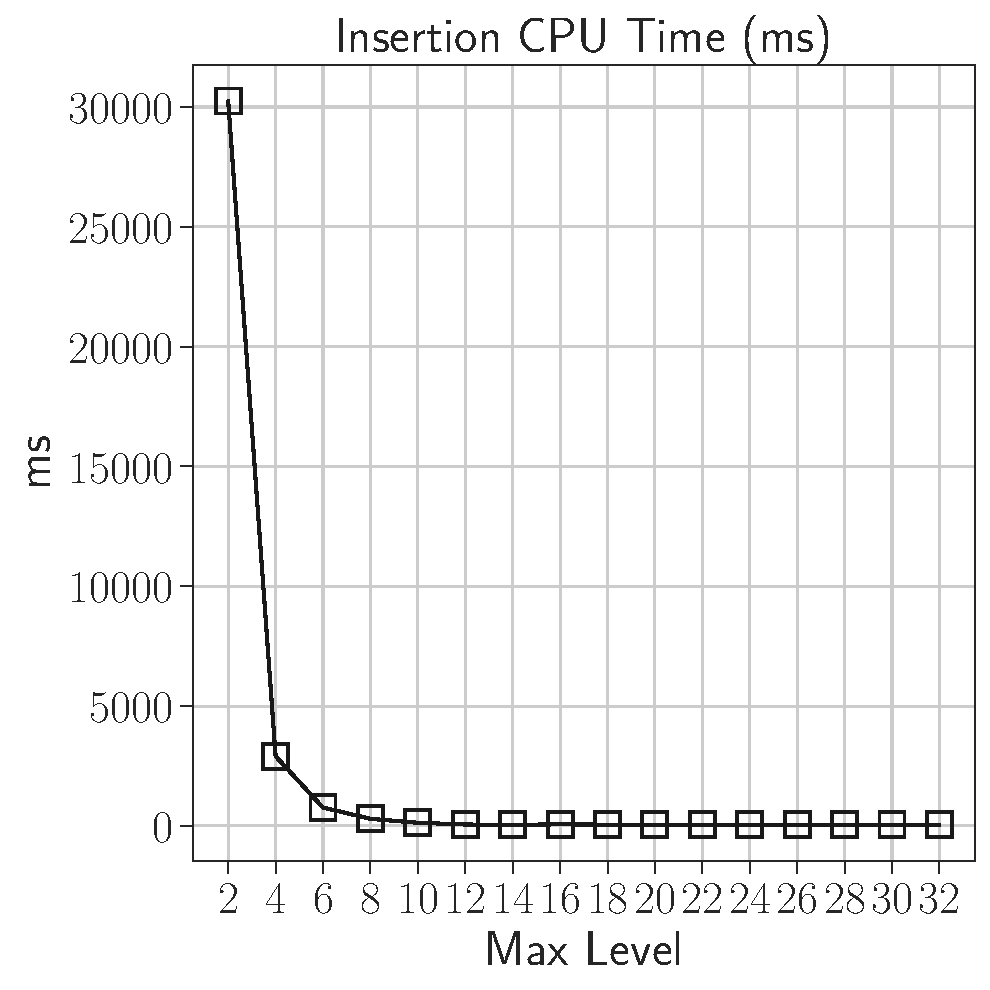
\includegraphics[width=\linewidth]{../notebook/plot/sl_maxlevel_insertion_cpu_time_(ms).pdf}
		\label{fig:cpu_time}
	\end{minipage}\hfill
	\begin{minipage}{0.32\textwidth}
		\centering
		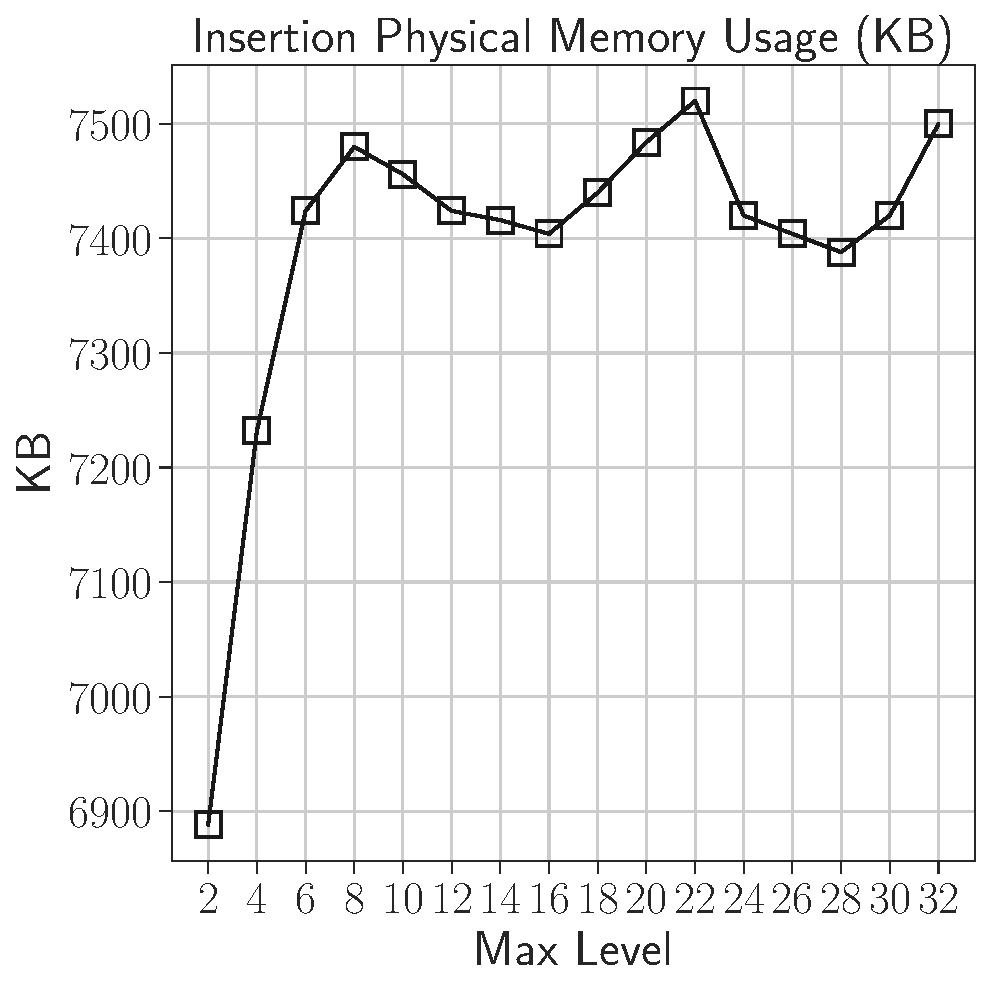
\includegraphics[width=\linewidth]{../notebook/plot/sl_maxlevel_insertion_physical_memory_usage_(kb).pdf}
		\label{fig:physical_memory}
	\end{minipage}\hfill\
	\begin{minipage}{0.32\textwidth}
		\centering
		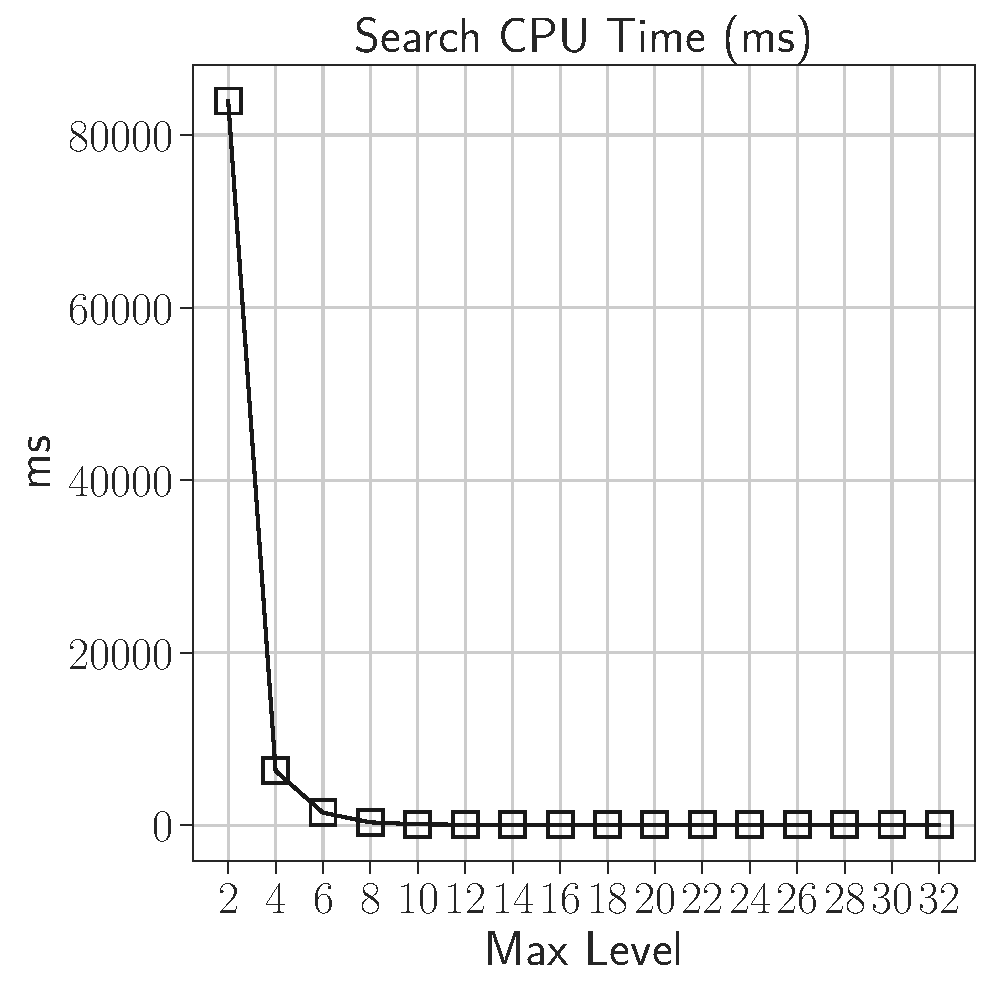
\includegraphics[width=\linewidth]{../notebook/plot/sl_maxlevel_search_cpu_time_(ms).pdf}
		\label{fig:physical_memory}
	\end{minipage}\hfill
	\caption{Crop of }
\end{figure}


b.) Search algorithm of Skip List when start is at the bottom left corner in $O(\log(d))$ where d is the number of elements smaller than the key?
	

	
	\vspace{2in} %Leave space for comments!
	
	
	\pagebreak
	\subsection*{Problem 8. ($a,b$) tree. ($2, 3$) tree.}

	a.)	
	\begin{figure}[H] 
		\centering
		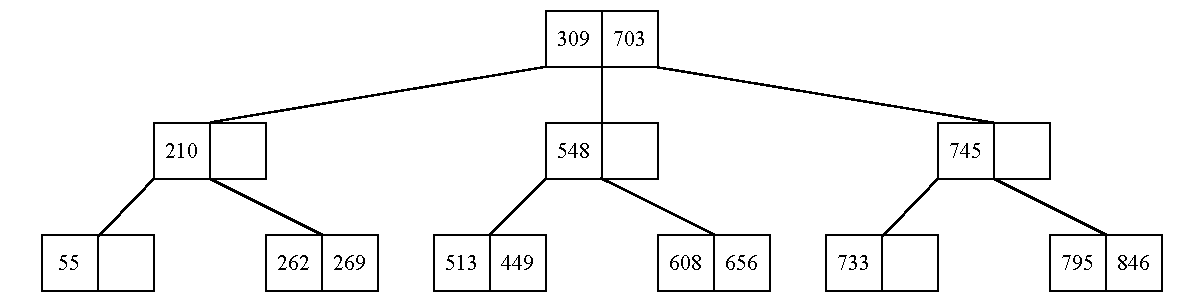
\includegraphics[width=0.9\linewidth]{Q8_a.drawio}
		\caption{Keys $733, 703, 608, 846, 309, 269, 55, 745, 548, 449, 513, 210, 795, 656, 262$ inserted into a $(2, 3)$ tree.}
		\label{fig:q8a}
	\end{figure}
	

	
	b.) 
	\begin{figure}[H] 
		\centering
		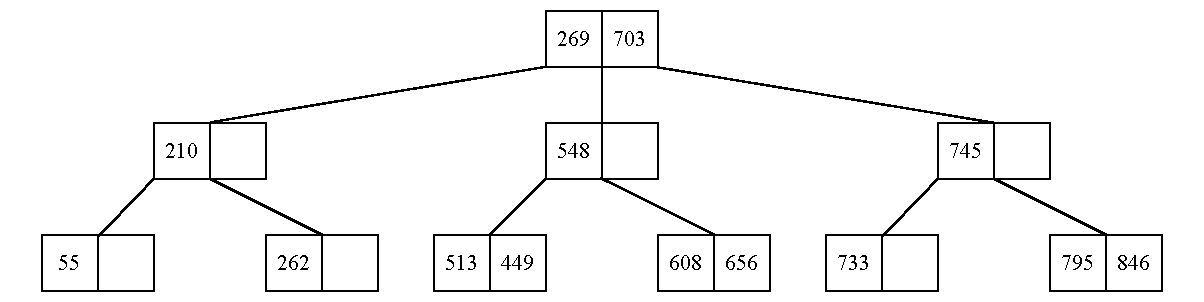
\includegraphics[width=0.9\linewidth]{Q8_b.drawio}
		\caption{Key 309 removed from Figure~\ref{fig:q8a} tree.}
		\label{fig:q8b}
	\end{figure}
	
	
\vspace{2in} %Leave space for comments!

\pagebreak
\subsection*{Problem 9. B-Tree Speed}

\subsubsection*{Experimental Setup}
Conducted our benchmarks using Google Benchmark~\cite{google-bench} on a system with the following hardware specifications:

\begin{itemize}
	\small
	\item \textbf{Processor}: 11th Gen Intel(R) Core(TM) i7-11370H 4C/8T CPU @ 3.3 GHz
	\item \textbf{Cache Hierarchy}:
	\begin{itemize}
		\item L1 Data: 48 KiB per core (\(\times 4\))
		\item L1 Instruction: 32 KiB per core (\(\times 4\))
		\item L2 Unified: 1280 KiB per core (\(\times 4\))
		\item L3 Unified: 12,288 KiB (shared)
	\end{itemize}
\end{itemize}

All benchmarks were compiled using \texttt{-Ox} optimization level with \texttt{MSVC} (version 19.42.34436) and executed in a single-threaded environment to minimize external interference. Memory usage was measured using the Windows API \texttt{GetProcessMemory()}~\cite{getprocessmemoryinfo}.\\
\\
The B-Tree implementation utilized in this experiment is sourced from the repository by frozenca
on GitHub~\cite{btree_github}.

\subsubsection*{Finding Optimal Parameter b Of B-Tree}
First I carried out benchmarks to measure performance, $20 \times 10^6$ random unique keys being inserted into the B-Tree while varying b parameter. Measured aggregate data, It is generally more stable than measure per operation. The operation per millisecond (ops/ms) is computed $\text{CPU-Time}/ 20 \times 10^6$.

\vspace{15pt}
\noindent
\begin{minipage}{1\textwidth}
    \centering
	\resizebox{0.7\textwidth}{!}{%
	\begin{tabular}{rrrr}
		\hline
		\textbf{b} & \textbf{ops/ms} & \textbf{CPU Time (ms)} & \textbf{Memory Usage (KB)} \\
		\hline
		2    & 336.93 & 59359.38  & 2544788 \\
		4    & 229.97 & 86968.75  & 1063908 \\
		6    & 187.82 & 106484.38 & 740108  \\
		8    & 162.25 & 123265.63 & 596900  \\
		16   & 147.98 & 135156.25 & 400248  \\
		32   & 138.27 & 144640.63 & 309792  \\
		64   & 130.08 & 153750.00 & 268680  \\
		128  & 122.46 & 163312.50 & 256996  \\
		256  & 114.90 & 174062.50 & 267676  \\
		512  & 107.48 & 186078.13 & 280852  \\
		1024 & 99.60  & 200796.88 & 285412  \\
		2048 & 90.49  & 221015.63 & 246636  \\
		\hline
	\end{tabular}
	}
	\captionof{table}{Benchmark results for B-Tree insertion with $20 \times 10^6$ inserts and varying $b$ from 2 to 2048.}
\end{minipage}%


\begin{figure}[H]
	\centering

	\begin{minipage}{0.5\textwidth}
		\centering
		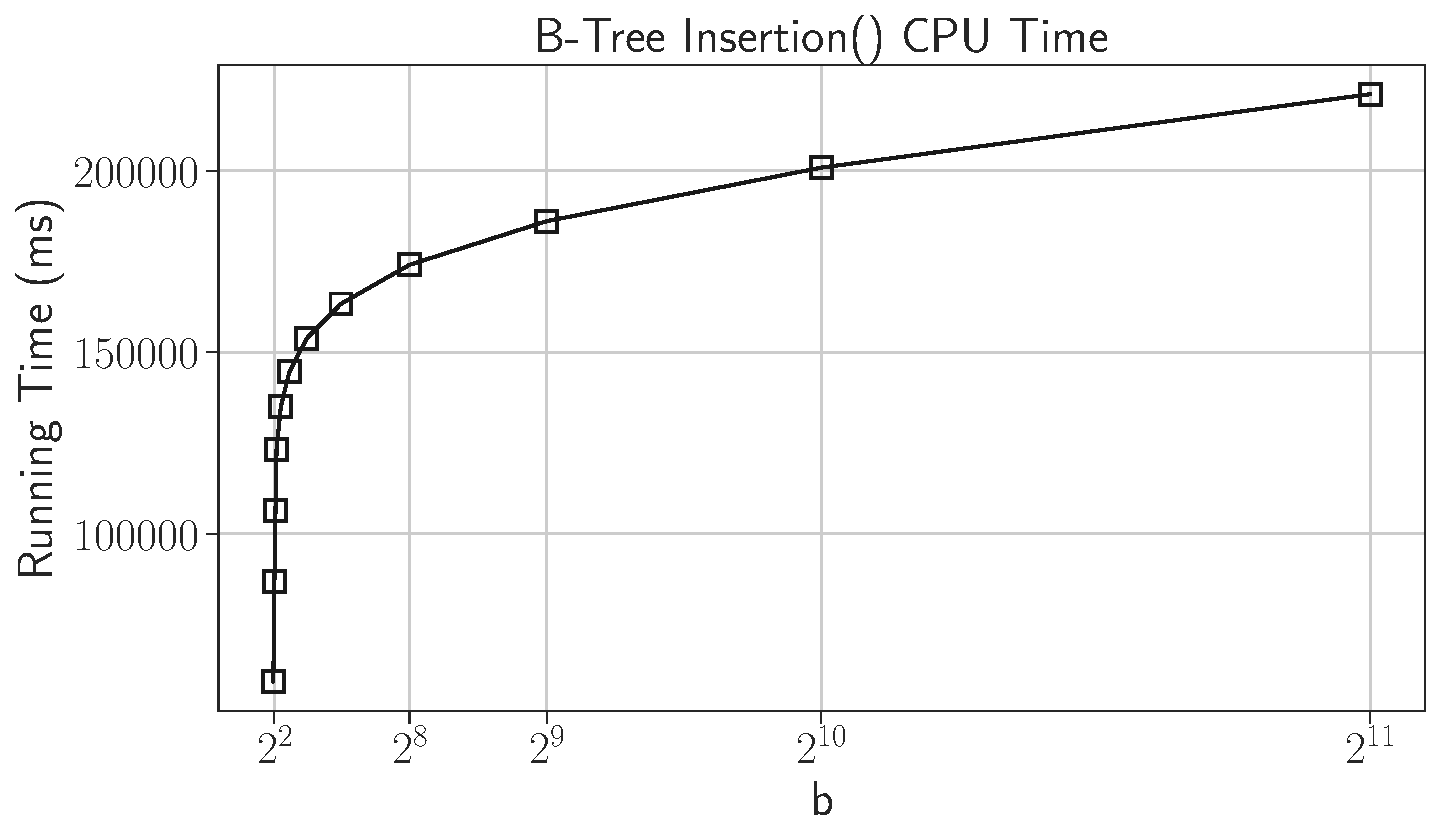
\includegraphics[width=\linewidth]{../notebook/plot/b-tree_insertion()_cpu_time.pdf}
		\label{fig:cpu_time}
	\end{minipage}\hfill
	\begin{minipage}{0.5\textwidth}
		\centering
		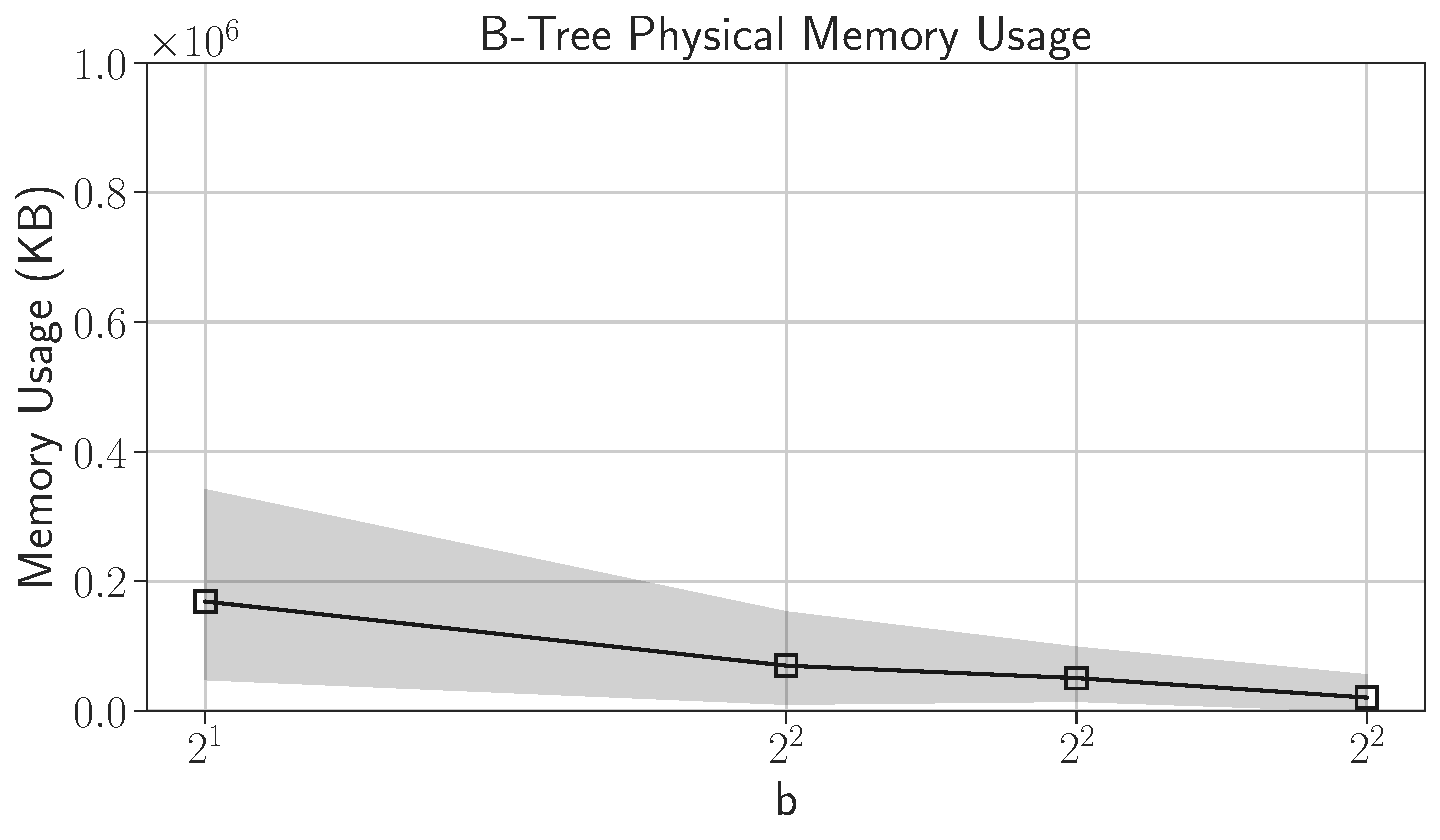
\includegraphics[width=\linewidth]{../notebook/plot/b-tree_physical_memory_usage.pdf}
		\label{fig:physical_memory}
	\end{minipage}\hfill
	\caption{CPU Time and Memory Usage for B-Tree insertion with varying $b$ values.}
\end{figure}

Notice that as the parameter of $b$ the B-Tree increases, the physical memory usage decreases. My theory is that increasing $b$ makes the tree shallower and more compact. Since a shallower tree reduces the number of pointers and improves spatial locality, nodes are more likely to fit within a cache line, leading to better memory efficiency?
\\\\
Anywhow... we want the b such that the it minimizes CPU time and memory used. They way I did it is to simply normalize CPU time and memory used and get closest b with to the smallest differnce. 

\begin{figure}[H]
	\centering
	\begin{minipage}{1\textwidth}
		\centering
		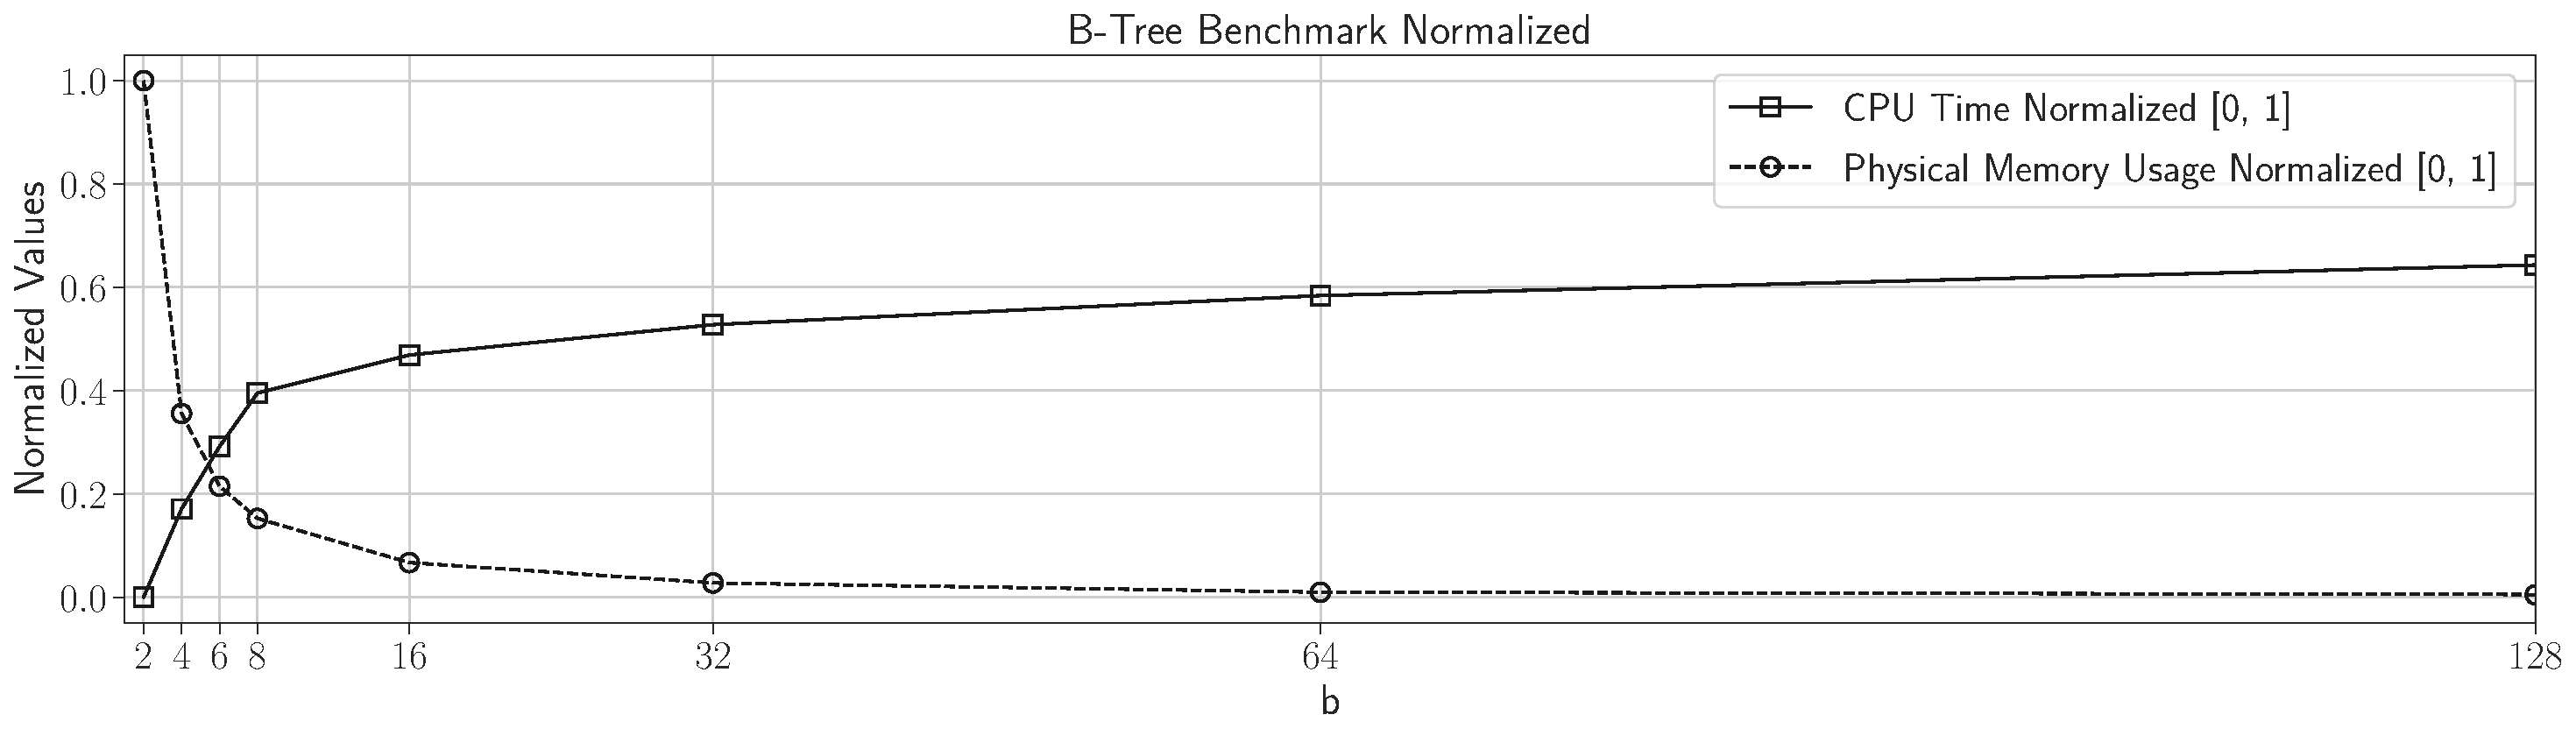
\includegraphics[width=\linewidth]{../notebook/plot/b-tree_benchmark_normalized.pdf}
		\label{fig:benchmark_normalized}
	\end{minipage}
	\caption{Normalized CPU Time and Memory Usage comparison for B-Tree insertion with varying $b$ values.}
\end{figure}

Setting $b = 6$ minimizes both performance overhead and memory usage the most. However, for applications that prioritize memory efficiency over execution time, a larger value, such as $b = 16$, may be more optimal, as the performance trade-off becomes less significant. This version clarifies that $b = 6$ minimizes both performance overhead and memory usage while improving the flow of the second sentence.

\subsubsection*{Comparing B-Tree and Builtin Ordered-Map Performance}


\begin{figure}[H]
	\centering
	\begin{minipage}{0.5\textwidth}
		\centering
		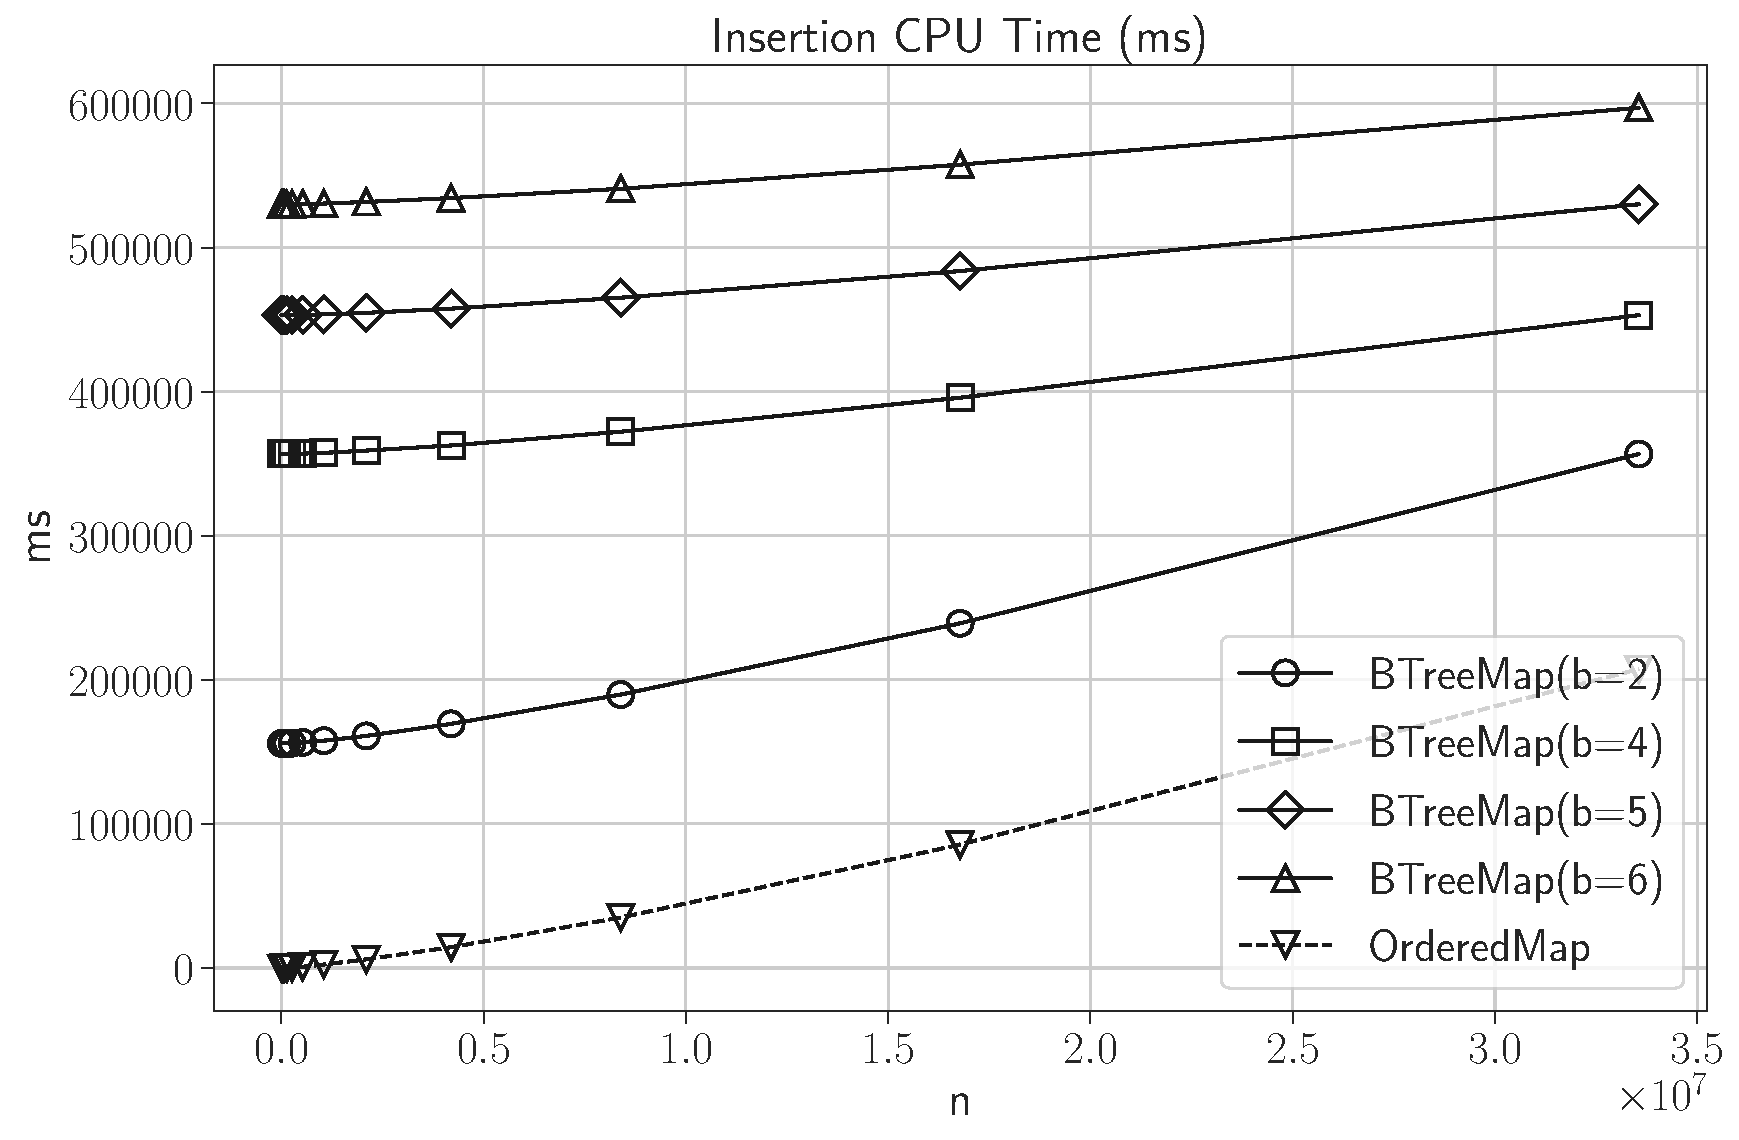
\includegraphics[width=1\linewidth]{../notebook/plot/insertion_cpu_time_(ms)}
	\end{minipage}\hfill
	\begin{minipage}{0.5\textwidth}
		\centering
		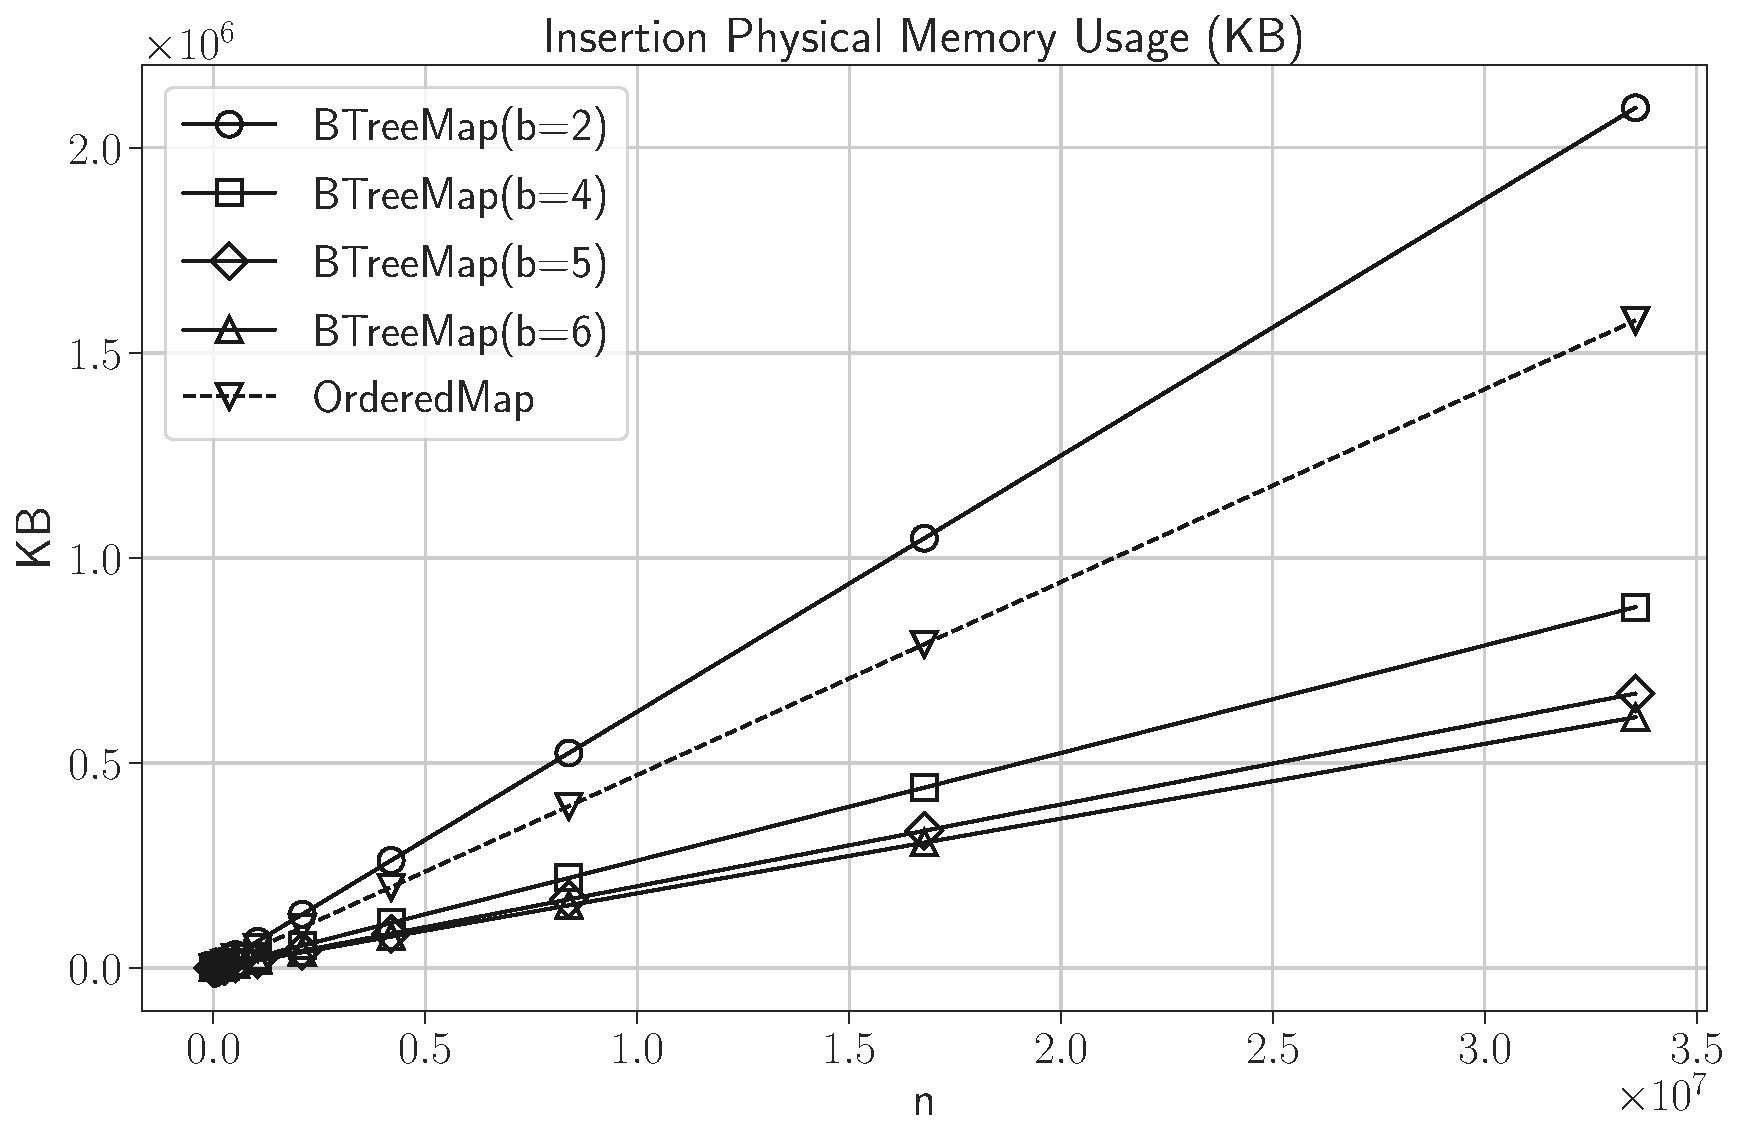
\includegraphics[width=1\linewidth]{../notebook/plot/insertion_physical_memory_usage_(kb)}
	\end{minipage}\hfill 
	\\
	\begin{minipage}{0.5\textwidth}
		\centering
		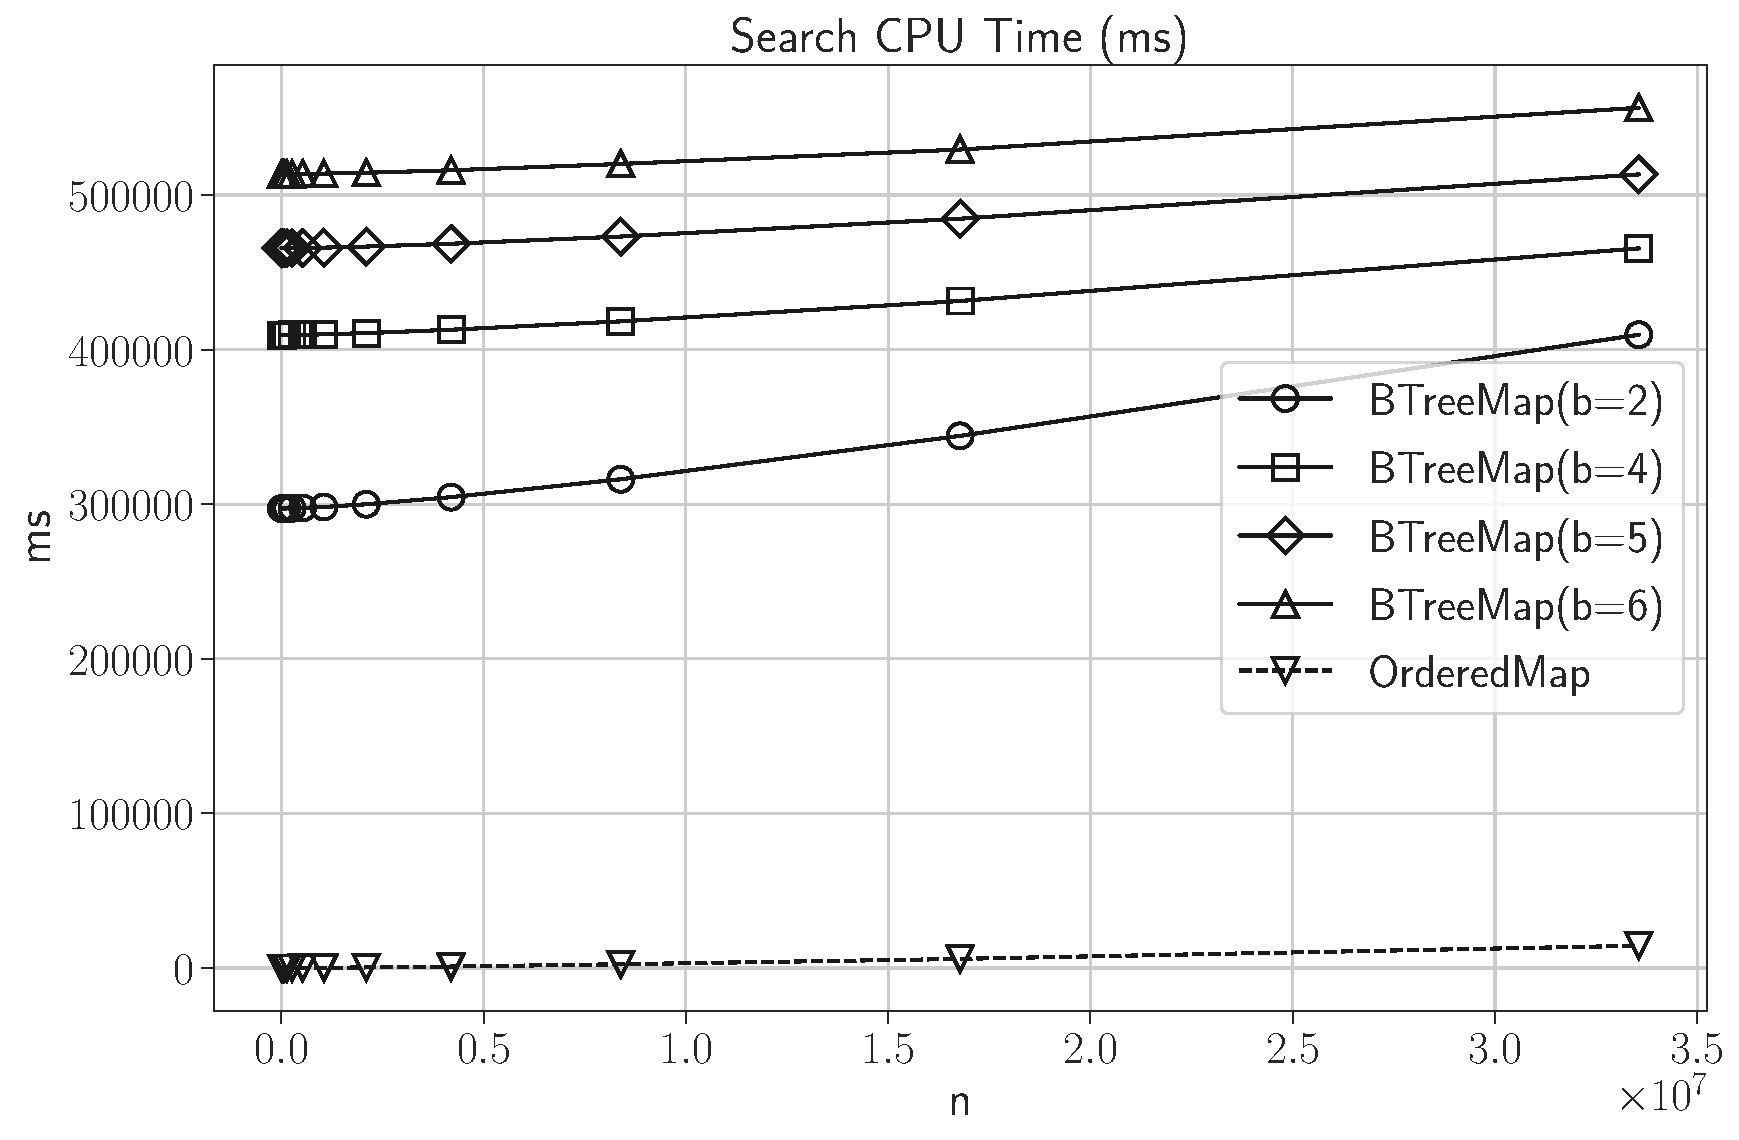
\includegraphics[width=1\linewidth]{../notebook/plot/search_cpu_time_(ms)}
	\end{minipage}\hfill

	\caption{CPU Time and Memory Usage of B-Tree and C++ Builtin Ordered Map. Inserted $2^{24}$ unique and random keys.}
	\label{fig:om_vs_bt}
\end{figure}




Figure~\ref{fig:om_vs_bt} illustrates that the running time for the C++ built-in Ordered Map outperforms the B-Tree in both insertion and search operations. However, it is important to note that for B-Trees with $b > 2$, memory efficiency improves, making them more memory-efficient than the built-in Ordered Map.


\noindent
\begin{minipage}{0.45\textwidth}
    \centering
	\resizebox{1\textwidth}{!}{%
		\begin{tabular}{rrr}
		\hline
		\multicolumn{3}{c}{\textbf{Ordered Map Insertion}} \\ \hline
		n             & CPU Time (ms)      & Memory Usage (KB)      \\ \hline
		8        & 0.00E+00 & 4       \\
		16       & 0.00E+00 & 0       \\
		32       & 0.00E+00 & 0       \\
		64       & 0.00E+00 & 0       \\
		128      & 0.00E+00 & 0       \\
		256      & 0.00E+00 & 4       \\
		512      & 0.00E+00 & 12      \\
		1024     & 0.00E+00 & 24      \\
		2048     & 0.00E+00 & 64      \\
		4096     & 0.00E+00 & 176     \\
		8192     & 0.00E+00 & 368     \\
		16384    & 3.13E+01 & 684     \\
		32768    & 1.56E+01 & 1584    \\
		65536    & 4.69E+01 & 3080    \\
		131072   & 1.41E+02 & 5936    \\
		262144   & 3.28E+02 & 11884   \\
		524288   & 8.91E+02 & 24628   \\
		1048576  & 2.42E+03 & 49260   \\
		2097152  & 6.02E+03 & 98572   \\
		4194304  & 1.44E+04 & 197348  \\
		8388608  & 3.51E+04 & 394748  \\
		16777216 & 8.57E+04 & 789744  \\
		33554432 & 2.08E+05 & 1579572 \\ \hline
		\end{tabular}
		}
\end{minipage}%
\hfill
\begin{minipage}{0.45\textwidth}
    \centering
	\resizebox{1\textwidth}{!}{%
		\begin{tabular}{rrr}
		\hline
		\multicolumn{3}{c}{\textbf{B-Tree $$b=6$$ Insertion}} \\ \hline
		n             & CPU Time (ms)      & Memory Usage (KB)      \\ \hline
		8        & 5.30E+05 & 4      \\
		16       & 5.30E+05 & 0      \\
		32       & 5.30E+05 & 0      \\
		64       & 5.30E+05 & 0      \\
		128      & 5.30E+05 & 4      \\
		256      & 5.30E+05 & 4      \\
		512      & 5.30E+05 & 8      \\
		1024     & 5.30E+05 & 16     \\
		2048     & 5.30E+05 & 32     \\
		4096     & 5.30E+05 & 68     \\
		8192     & 5.30E+05 & 124    \\
		16384    & 5.30E+05 & 308    \\
		32768    & 5.30E+05 & 576    \\
		65536    & 5.30E+05 & 1148   \\
		131072   & 5.30E+05 & 2216   \\
		262144   & 5.30E+05 & 4460   \\
		524288   & 5.30E+05 & 9356   \\
		1048576  & 5.31E+05 & 19092  \\
		2097152  & 5.32E+05 & 38316  \\
		4194304  & 5.34E+05 & 76508  \\
		8388608  & 5.41E+05 & 152888 \\
		16777216 & 5.58E+05 & 305684 \\
		33554432 & 5.97E+05 & 611656  \\ \hline
		\end{tabular}
	}
    % \captionof{table}{First Table}
\end{minipage}%

\vspace{14pt}

\noindent
\begin{minipage}{0.45\textwidth}
    \centering
	\resizebox{1\textwidth}{!}{%
		\begin{tabular}{rrr}
		\hline
		\multicolumn{3}{c}{\textbf{Ordered Map Search}} \\ \hline
		n             & CPU Time (ms)      & Memory Usage (KB)      \\ \hline
		8        & 3.07E-05 & 4       \\
		16       & 7.67E-05 & 0       \\
		32       & 1.71E-04 & 0       \\
		64       & 4.53E-04 & 0       \\
		128      & 9.63E-04 & 0       \\
		256      & 2.22E-03 & 4       \\
		512      & 4.46E-03 & 12      \\
		1024     & 2.93E-02 & 24      \\
		2048     & 9.42E-02 & 64      \\
		4096     & 2.68E-01 & 176     \\
		8192     & 6.28E-01 & 368     \\
		16384    & 1.38E+00 & 684     \\
		32768    & 3.29E+00 & 1584    \\
		65536    & 8.54E+00 & 3080    \\
		131072   & 2.34E+01 & 5936    \\
		262144   & 1.02E+02 & 11884   \\
		524288   & 2.66E+02 & 24628   \\
		1048576  & 8.13E+02 & 49260   \\
		2097152  & 2.06E+03 & 98572   \\
		4194304  & 5.06E+03 & 197348  \\
		8388608  & 1.43E+04 & 394748  \\
		16777216 & 3.06E+04 & 789744  \\
		33554432 & 7.36E+04 & 1579572 \\ \hline
		\end{tabular}
	}
\end{minipage}%
\hfill
\begin{minipage}{0.45\textwidth}
    \centering
	\resizebox{1\textwidth}{!}{%
		\begin{tabular}{rrr}
		\hline
		\multicolumn{3}{c}{\textbf{B-Tree $$b=6$$ Search}} \\ \hline
		n             & CPU Time (ms)      & Memory Usage (KB)      \\ \hline
		8        & 1.66E+06 & 4      \\
		16       & 1.66E+06 & 0      \\
		32       & 1.66E+06 & 0      \\
		64       & 1.66E+06 & 0      \\
		128      & 1.66E+06 & 4      \\
		256      & 1.66E+06 & 4      \\
		512      & 1.66E+06 & 8      \\
		1024     & 1.66E+06 & 16     \\
		2048     & 1.66E+06 & 32     \\
		4096     & 1.66E+06 & 68     \\
		8192     & 1.66E+06 & 124    \\
		16384    & 1.66E+06 & 308    \\
		32768    & 1.66E+06 & 576    \\
		65536    & 1.66E+06 & 1148   \\
		131072   & 1.66E+06 & 2216   \\
		262144   & 1.66E+06 & 4460   \\
		524288   & 1.66E+06 & 9356   \\
		1048576  & 1.66E+06 & 19092  \\
		2097152  & 1.66E+06 & 38316  \\
		4194304  & 1.67E+06 & 76508  \\
		8388608  & 1.68E+06 & 152888 \\
		16777216 & 1.72E+06 & 305684 \\
		33554432 & 1.81E+06 & 611656  \\ \hline
		\end{tabular}
	}
    % \captionof{table}{First Table}
\end{minipage}%

\vspace{14pt}


\begin{thebibliography}{9}
	\bibitem{google-bench} 
	Google Benchmark. 
	\textit{A microbenchmark support library}. \\
	\url{https://github.com/google/benchmark}

	\bibitem{btree_github} 
	B-Tree Implementation on GitHub. 
	\textit{GitHub Repository}. \\
	\url{https://github.com/frozenca/BTree}

	\bibitem{getprocessmemoryinfo} 
	GetProcessMemoryInfo function. 
	\textit{Microsoft Learn}. \\
	\url{https://learn.microsoft.com/en-us/windows/win32/api/psapi/nf-psapi-getprocessmemoryinfo}

	\bibitem{stack-overflow} 
	Skip Lists Stack Overflow.
	\sloppy\url{https://stackoverflow.com/questions/31580869/skip-lists-are-they-really-performing-as-good-as-pugh-paper-claim/34003558\#34003558}

\end{thebibliography}

	
\end{document}